% !TEX TS-program = xeLaTeX+MakeIndex+BibTeX 
\newcommand{\tabincell}[2]{\begin{tabular}{@{}#1@{}}#2\end{tabular}}
\documentclass[xcolor=x11names,compress]{beamer}
\usetheme{Darmstadt} 
\useoutertheme[subsection=false,footline=authortitle]{miniframes}
\setbeamertemplate{navigation symbols}{} 

\setbeamercolor*{lower separation line head}{bg=DeepSkyBlue4} 
\setbeamercolor*{normal text}{fg=black,bg=white} 
\setbeamercolor*{alerted text}{fg=red} 
\setbeamercolor*{example text}{fg=black} 
\setbeamercolor*{structure}{fg=DeepSkyBlue4,bg=white} 

\setbeamercolor*{palette tertiary}{fg=black,bg=black!10} 
\setbeamercolor*{palette quaternary}{fg=black,bg=black!10} 

%footline
\setbeamercolor{author in head/foot}{fg=white,bg=}
\setbeamercolor{title in head/foot}{fg=white,bg=}
\setbeamercolor{date in head/foot}{fg=black,bg=}


\makeatletter
\setbeamertemplate{footline}
{%
    \setbox\beamer@tempbox=\hbox{%
        \begin{beamercolorbox}[wd=.333333\paperwidth,ht=2.25ex,dp=1ex,center]{author in head/foot}%
            \usebeamerfont{author in head/foot}\insertshortauthor
        \end{beamercolorbox}%
        \begin{beamercolorbox}[wd=.333333\paperwidth,ht=2.25ex,dp=1ex,center]{title in head/foot}%
            \usebeamerfont{title in head/foot}\insertshorttitle
        \end{beamercolorbox}%
        \begin{beamercolorbox}[wd=.333333\paperwidth,ht=2.25ex,dp=1ex,right]{date in head/foot}%
            \usebeamerfont{date in head/foot}\insertshortdate{}\hspace*{2em}
            \insertframenumber{} / \inserttotalframenumber\hspace*{2ex} 
        \end{beamercolorbox}%
    }%
    \vskip0pt%
        \begin{pgfpicture}{0pt}{0pt}{\paperwidth}{0cm}%
            \usebeamercolor{frametitle right}%
            \pgfpathrectangle{\pgfpointorigin}{\pgfpoint{\paperwidth}{3.5ex}}%
            \pgfusepath{clip}%
            \pgftext[left,base]{\pgfuseshading{beamer@frametitleshade}}%
        \end{pgfpicture}%
    \beamer@tempdim=\ht\beamer@tempbox%
    \advance\beamer@tempdim by 0.95ex%
    \vskip-\beamer@tempdim%
    \box\beamer@tempbox%
    }  
\makeatother


\colorlet{titleright}{yellow!10!white}
\colorlet{titleleft}{DeepSkyBlue4}
\colorlet{titlemid}{green!60!blue}

\makeatletter

\pgfdeclarehorizontalshading[titleleft,titleright]{beamer@frametitleshade}{\paperheight}{%
        color(0pt)=(titleleft);
        color(.5\paperwidth)=(titlemid);
        color(\paperwidth)=(titleright)
}

\AtBeginDocument{
    \pgfdeclareverticalshading{beamer@topshade}{\paperwidth}{%
        color(0pt)=(bg);
        color(4pt)=(black!50!bg)    
    }
}


\renewcommand{\(}{\begin{columns}}
\renewcommand{\)}{\end{columns}}
\newcommand{\<}[1]{\begin{column}{#1}}
\renewcommand{\>}{\end{column}}


\usepackage{graphicx}
\usepackage{subfigure} 
\usepackage{color}
\usepackage{ragged2e}
\renewcommand{\raggedright}{\leftskip=0pt \rightskip=0pt plus 0cm}
\title{Hedging Climate Change News}

\author[Engle et al.]{R. Engle, S. Giglio, B. Kelly, H. Lee and J. Stroebel}

\institute{}

\date{\today}

\begin{document}
	
	\maketitle
	\begin{frame}<beamer>
		\frametitle{Outline}
		\tableofcontents[hideallsubsections]
	\end{frame}
	
	\AtBeginSection[]
	{
		\begin{frame}<beamer>
			\frametitle{Outline}
			\tableofcontents[currentsection,hideothersubsections]
		\end{frame}
	}
	\AtBeginSubsection[]
	{
		\begin{frame}[shrink]
			\frametitle{Outline}
			\tableofcontents[sectionstyle=show/hide,subsectionstyle=show/shaded/hide]
		\end{frame}
	}

\section{Introduction on climate finance}

\begin{frame}{Introduction}{Climate finance}
	\begin{itemize}
		\item \textbf{Climate finance} is defined by the United Nations Framework Convention on Climate Change (UNFCCC) to be “local, national, or transnational financing—drawn from public, private, and alternative sources of financing—that seeks to support mitigation and adaptation actions that will address climate change.” 
		
	\end{itemize}	
\end{frame}
	
\section{This paper}
\begin{frame}{Introduction}
	\begin{itemize}
		\item Propose an approach for constructing climate risk hedge portfolios using publicly traded assets——constructing portfolios whose short-term returns hedge news about climate change over the holding period.
		\item \textbf{Method}: Mimicking portfolio approach
		\item \textbf{Portfolio}: Industry-balanced
		\item \textbf{Performance}: Perform well both in sample and out-of-sample
	\end{itemize}
\end{frame}
	
\begin{frame}{Background}
	\begin{itemize}
		\item Uncertainty around the trajectory and the economic consequences of climate change is substantial.
		\item Investors desire to hedge against climate risk.
		\item Because of the long run and nondiversifiable nature of climate risk, standard futures or insurance contracts are difficult to implement	
	\end{itemize}
\end{frame}
	
\begin{frame}{Outline}{Step 1}
	\begin{itemize}
		\item \textbf{Step 1}: Construct a time series that captures news about long-run climate risk
		\item [-] \textbf{Index 1}: The correlation between the text content of the Wall Street Journal and a fixed climate change vocabulary
		\item [-] \textbf{Index 2}: Applying sentiment analysis to climate-related articles to measure the intensity of negative climate news in a given month.
		\item [-]Do not try to distinguish between different types of climate change news.
		\item [-]Ignore news about local climate events
	\end{itemize}	
\end{frame}
	
\begin{frame}{Outline}{Step 2}
	\begin{itemize}
		\item \textbf{Step 2}: Construct portfolios to hedge innovations in the two news series
		\item [-] \textbf{Goal}: Investors can hedge their climate risk exposure by trading this portfolio without changing their exposures to the other risk factors in their portfolios.
		\item [-] \textbf{A concern}: Data mining. We only observe a limited number of months of climate news realizations, but have a large set of assets that we could use to form the hedge portfolio.
		\item [-] \textbf{The solution}: Use characteristics that proxy for a firm's exposure to climate risk to parameterize the weights of the hedge portfolios. Characteristics: firm-level environmental performance score
	\end{itemize}	
\end{frame}

\begin{frame}{Outline}{Step 3}
	\begin{itemize}
		\item \textbf{Step 3}: Compare our hedge portfolios to alternative portfolios that add simple industry bets (energy ETF and clean energy ETF)
		\item [-] Our hedge portfolio do not resemble industry bets, and identify firms with the largest exposure to climate change risk both within and across industries.
		\item [-] The in-sample fit of our hedge portfolio is higher.
	\end{itemize}	
\end{frame}


\section{Theory}

\begin{frame}{Theory}{Mimicking portfolio approach}
	\begin{itemize}		
		\item Firm-level characteristics $Z_{t}$ include:
		\item [-] Climate characteristics (Firm-level normalized environmental performance score)
		\item [-] Size (standardized market value)
		\item [-] Value (Standardized book-to-market ratio)
		\item [-] Market (The share of total market value)
		\item The final regression equation becomes:
		$$
		\begin{aligned}
		C C_{t}=& \xi+w_{S U S} Z_{t-1}^{S U S_{-} A^{\prime}} r_{t}+w_{S I Z E} Z_{t-1}^{S I Z E^{\prime}} r_{t}+w_{H M L} Z_{t-1}^{H M L^{\prime}} r_{t} \\
		&+w_{M K T} Z_{t-1}^{M K T^{\prime}} r_{t}+e_{t}
		\end{aligned}
		$$
		\item [-] $r_{t}$: Excess returns of individual stocks
		\item [-]  $Z_{t}$: Normalized firm-level
	\end{itemize}	
\end{frame}

\section{Data}
\begin{frame}{Data on climate change news}{\textit{The Wall Street Journal} climate news index}
	\begin{itemize}		
		\item To quantify the intensity of climate news coverage in \textit{The Wall Street Journal} (WSJ), we compare the news content to a corpus of authoritative texts on the subject of climate change. 
		\item Next, we convert WSJ term counts into “term frequency–inverse document frequency” (\textit{tf-idf}) scores.
	\end{itemize}	
\end{frame}

\begin{frame}{Data on climate change news}{\textit{The Wall Street Journal} climate news index}
	\textbf{Term frequency–inverse document frequency (\textit{tf-idf})}
	\begin{itemize}		
		\item For a word $j$ in document $i$, term frequency $\left(t f_{i j}\right)$ is the count $c_{i j}$ of occurrences of $j$ in $i$. 
		\item Inverse document frequency $i d f_{j}$ is the log of one over the share of documents containing $j$. 
		\item The object of interest tf-idf is the product $t f_{i j} \times i d f_{j}$. 
		\item \textbf{Low $idf$ terms:} Common terms that appear in most documents, because they are less informative about any individual document’s content. 
		\item \textbf{Low $tf$ terms:} Terms that are rare in a given article.
		\item The \textit{tf-idf} transformation defines the most representative terms in a given document to be those that appear infrequently overall, but frequently in that specific document.
	\end{itemize}	
\end{frame}

\begin{frame}{Data on climate change news}{Crimson Hexagon’s negative sentiment climate change news index}
	\begin{itemize}		
		\item Using $Wall$ $Street$ $Journal$ climate news index has the risk of inaccurately capturing discussions of positive climate news as 		increases in climate risk.
		\item We use the services of the data analytics vendor \textbf{Crimson Hexagon}.
		\item Crimson Hexagon provided us with an array of indices that summarize the total number of articles that include climate change news, as well as the fraction of those summarized to contain positive and negative climate change news.
	\end{itemize}	
\end{frame}

\begin{frame}{Data on climate change news}{Constructing hedge targets}
 	\begin{itemize}		
 	\item The dependent variable, $C C_{t}$ is residuals from an AR(1) model of the two news series. 
 	\item The two monthly hedge targets are: 
 	\item [-] $C C_{t}^{W S J}$, which captures innovations in the WSJ Climate Change News Index
 	\item [-] $C C_{t}^{\text {NegNews }}$, which captures innovations in the CH Negative Climate Change News Index
 \end{itemize}
\end{frame}

\begin{frame}{Data on potential assets in hedge portfolios}
	\begin{itemize}		
		\item We focus on constructing hedge portfolios using U.S. equities as the underlying assets.
	\end{itemize}
\end{frame}

\begin{frame}{Data on climate risk exposures}{MSCI}
	\textbf{MSCI} evaluates firms along several subcategories that capture either positive or negative environmental performance.
	\begin{itemize}	
		\item We calculate an overall environmental score for each firm by subtracting the total scores in the negative environmental subcategories from the total scores in positive ones.
	\end{itemize}
	\textbf{Sustainalytics} provided us with monthly firm-level ESG scores beginning in September 2009.
	\begin{itemize}
		\item We use the “Total Environment Score” in our empirical analysis.
	\end{itemize}
\end{frame}

\begin{frame}{Data on climate risk exposures}{Data issues}
	\begin{figure}[hbdp]
		\centering
		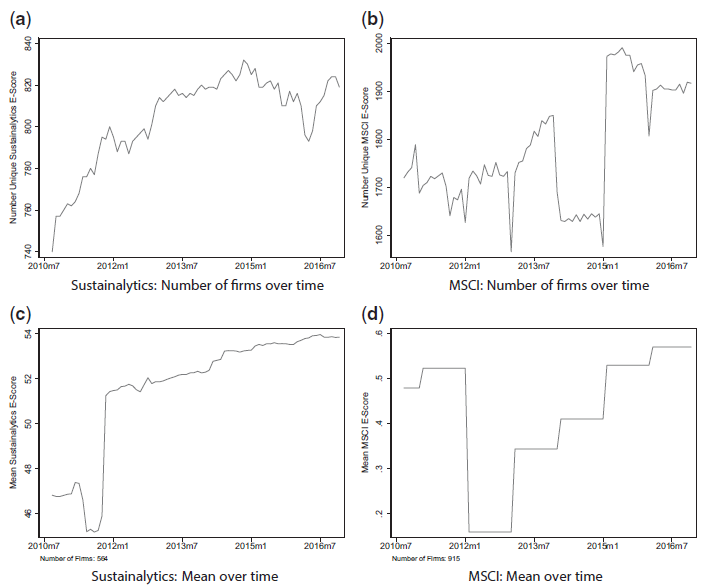
\includegraphics[width=0.7\textwidth]{performance.png}
	\end{figure} 
\end{frame}

\begin{frame}{Data on climate risk exposures}{Data issues}
	The averages of each score contain a number of discontinuous breaks.
	\begin{itemize}
		\item \textbf{Solution 1}: To minimize the complications from any modeling changes, we construct
		$Z_t$ by cross-sectionally demeaning each E-Score in each month.
		\item [-] Implicit assumption: Changes to the model shift the mean of the E-Scores over time. 
		\item \textbf{Solution 2}: We rank the E-Scores of all firms at each point in time, and then demean and rescale the ranked measure such that it ranges from -0.5 to +0.5.
		\item [-] Implicit assumption: Changes to the model shift the mean of the E-Scores over time, and the cross-sectional dispersion.
	\end{itemize} 
\end{frame}

\section{Results}
\begin{frame}{Forming hedge portfolios}
	We can use the following regression to estimate the weights of different stocks in the hedge portfolio:
	$$
	\begin{aligned}
	C C_{t}=& \xi+w_{S U S} Z_{t-1}^{S U S_{-} A^{\prime}} r_{t}+w_{S I Z E} Z_{t-1}^{S I Z E^{\prime}} r_{t}+w_{H M L} Z_{t-1}^{H M L^{\prime}} r_{t} \\
	&+w_{M K T} Z_{t-1}^{M K T^{\prime}} r_{t}+e_{t}
	\end{aligned}
	$$
	where $w_{S U S}, w_{S I Z E}, w_{H M L}$ and $w_{M K T}$ are scalars that capture the weight of the corresponding portfolios in the mimicking (hedge) portfolio for $C C_{t}.$
	\medskip
	 
	We also analyze the performance of hedge portfolios constructed using returns of the energy ETF and clean energy ETF instead of the returns of portfolios of stocks sorted by their E-Scores. 
\end{frame}

\begin{frame}{In-sample fit results}{Full-sample regression: WSJ Climate Change News Index}
	\begin{figure}[hbdp]
		\centering
		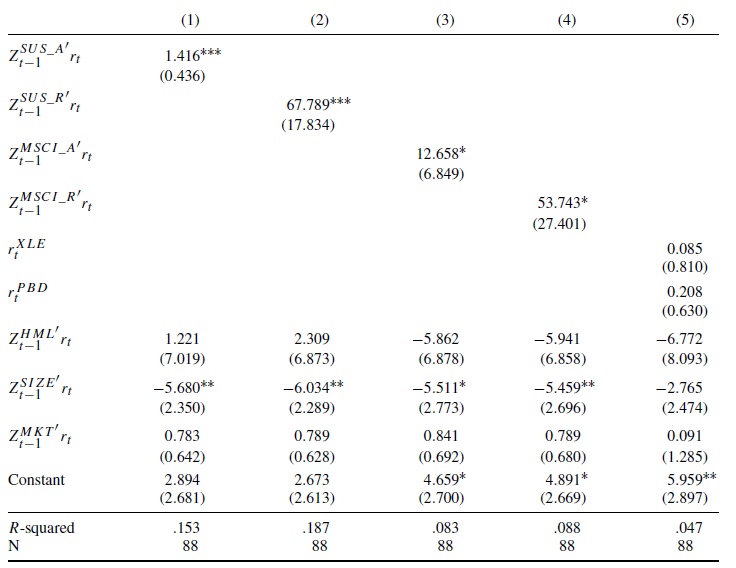
\includegraphics[width=0.84\textwidth]{tab1.png}
	\end{figure}
\end{frame}

\begin{frame}{In-sample fit results}{Full-sample regression: CH Negative Climate Change News Index}
	\begin{figure}[hbdp]
		\centering
		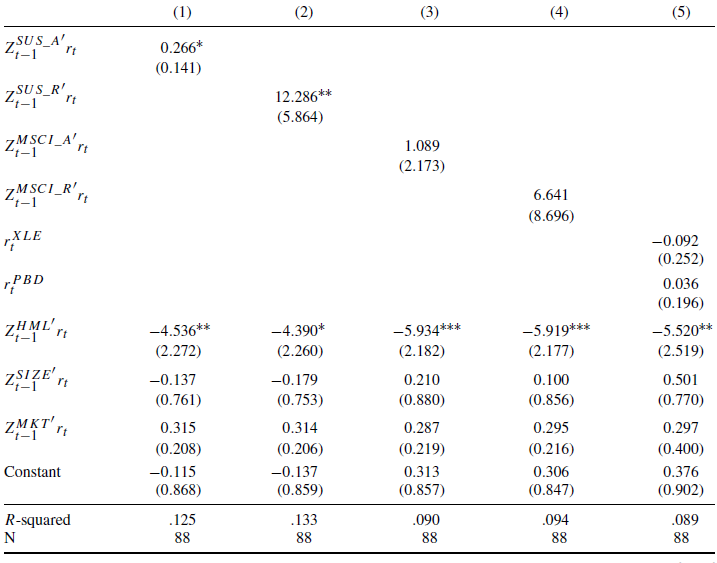
\includegraphics[width=0.8\textwidth]{tab2.png}
	\end{figure} 
\end{frame}

\begin{frame}{Out-of-sample fit results}
	The most important test of the hedge portfolios is their ability to hedge out-of-sample innovations to climate news.
	\medskip

	\begin{itemize}
		\item \textbf{Out-of-sample fit approach}: For every period $t$ we run regression using data between periods $t_{\min }$ and $t-1$\footnote{$t_{\min }$ corresponds to the first month for which we observe all climate exposures and $C C_{t}$ series (September $\left.2009\right)$.\\}. We then form the hedge portfolio based on these estimates and explore the correlation of the returns of that hedge portfolio in period $t$ with $C C_{t} .$ 
		\item \textbf{Cross-validation approach}: For every period $t^{\prime}$ we run the regression for all periods $t \neq t^{\prime},$ and then use the resultant estimates to construct hedge portfolio.
	\end{itemize}	 
\end{frame}

\begin{frame}{Out-of-sample fit results}{Cross-correlations: WSJ Climate Change News Index}
	\begin{figure}[hbdp]
	\centering
	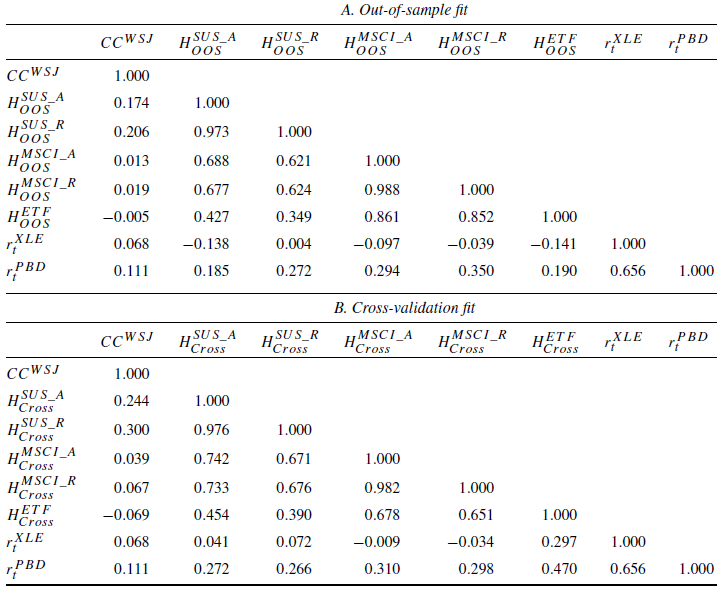
\includegraphics[width=0.7\textwidth]{tab4.png}
	\end{figure} 	 
\end{frame}

\section{Conclusion and directions}

\begin{frame}{Conclusion}
	\begin{itemize}
	\item We demonstrate how a mimicking portfolio approach can be successful in hedging innovations in climate change news across a number of out-of-sample performance tests. 
	\item The hedge portfolios based on Sustainalytics E-Scores have the best in-sample fit as well as the best out-of-sample and cross-validation performance. Portfolios based on MSCI EScores and ETFs have a lower (but still positive) ability to hedge innovations in climate news. 
	\item There are no systematic differences in the relative performance of hedge portfolios based on absolute or ranked versions of the raw E-Scores.
	\end{itemize}	
\end{frame}

\begin{frame}{Directions for future research}
	Future research in the field of climate finance may consider the addition of more assets to the hedge portfolios and the formation of hedge portfolios based on both characteristic-sorted portfolios and ETFs.
	\medskip

	\begin{itemize}
	\item E.g.1: Integrate more and better data to measure firm-level climate risk exposures.
	\item E.g.2: Develop alternative definitions of the climate change risks. One interesting question is whether it is important to differentiate between physical and policy-oriented climate risks.
	\item E.g.3: A related question pertains to the expected returns of the various hedge portfolios.
	\end{itemize}
\end{frame}

\end{document}